\section{Design}

\subsection{Overview}

\system is a host-side placement layer for \zns devices.  Figure~\ref{fig:architecture} shows the data path.  Applications or cryptographic libraries produce lifecycle labels when they create PQC artifacts.  These labels are attached to writes as \texttt{quasar\_hint}.  The allocator maps each write to a zone family.  An epoch manager tracks which families are eligible for reset, migration, or fallback GC.  Payload writes continue to use a history-based fallback, so the system does not discard the strengths of \dogi-style placement.

\begin{figure*}[t]
\centering
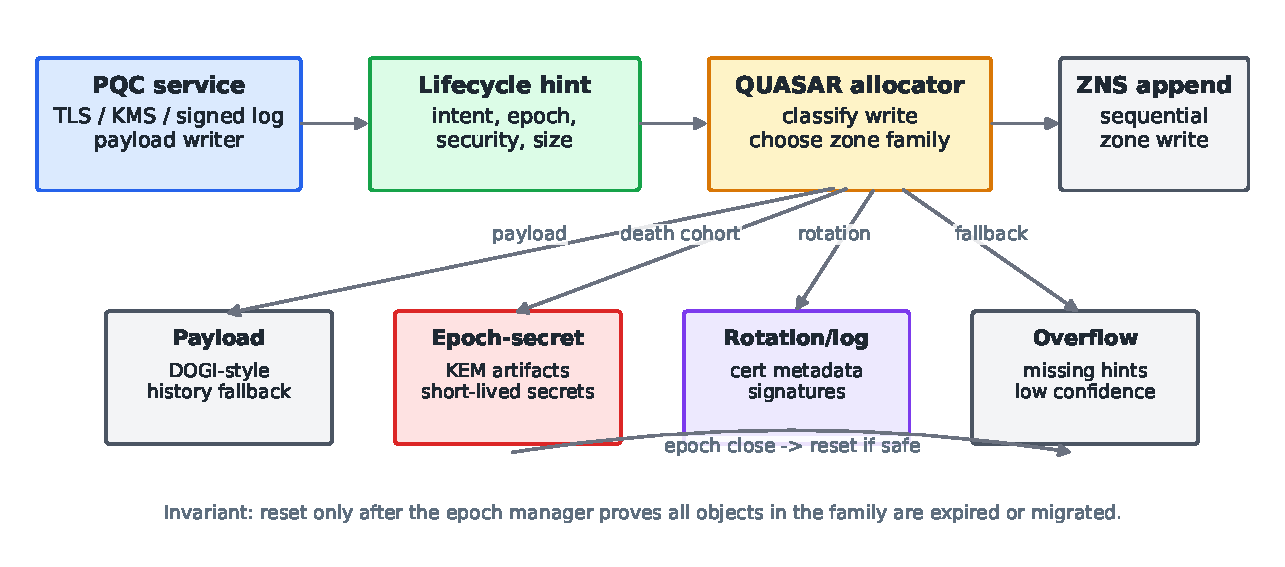
\includegraphics[width=0.86\textwidth]{../artifacts/figures/paper/quasar-architecture.pdf}
\caption{\system architecture.  The storage path receives lifecycle labels, not secret material.  Payload remains on a history-based fallback, while PQC secrets, rotation metadata, and uncertain writes are routed to separate zone families.  The epoch manager resets or sanitizes a family only after proving that all objects in the family are expired or migrated.}
\label{fig:architecture}
\end{figure*}

\subsection{Design Requirements}

\system follows the three requirements from Motivation.  Lifecycle labels expose protocol lifetime and route PQC objects to death-cohort zone families while payload stays on \dogi-style fallback.  Admission control budgets exact placement by reserving scarce exact families for high-security secrets and sending sparse or uncertain writes to bins or overflow.  Epoch-confirmed reclaim resets a family only after durable epoch close or residual migration; uncertain zones fall back to normal GC.  The evaluation checks these requirements with stale-secret exposure rows, pressure traces, multi-tenant stress, bad hints, and sanitize-boundary tests.

\subsection{Hint Schema}

The hint is intentionally small.  It contains only lifecycle metadata:

\begin{lstlisting}[language=C,caption={Minimal \system hint schema.},label={lst:hint}]
enum quasar_intent {
  QUASAR_PAYLOAD = 0,
  QUASAR_EPHEMERAL_SECRET = 1,
  QUASAR_KEM_ARTIFACT = 2,
  QUASAR_SIGNATURE_LOG = 3,
  QUASAR_CERT_METADATA = 4,
};

struct quasar_hint {
  uint16_t intent;
  uint16_t expire_class;
  uint32_t security_class;
  uint64_t epoch_id;
  uint64_t cohort_id;
  uint64_t size_bytes;
};
\end{lstlisting}

The fields are lifecycle labels, not cryptographic secrets.  \texttt{intent} separates secrets, KEM artifacts, signature logs, certificate metadata, and payload.  \texttt{epoch\_id} identifies the death cohort.  \texttt{security\_class} sets reset urgency and isolation.  \texttt{cohort\_id} is opaque to storage and can be a keyed hash, so raw session, tenant, or key identifiers need not cross the storage boundary.

\noindent\textbf{Trust boundary.}
\system assumes that high-priority lifecycle hints are emitted by trusted components such as the TLS terminator, KMS, logging service, or a privileged policy layer.  Untrusted tenants do not directly grant themselves exact secret-zone priority.  A deployment can enforce per-tenant exact-family quotas, tenant-local cohort namespaces, and admission limits before a hint reaches the allocator.  If provenance is missing or confidence is low, the write is routed to overflow and becomes a performance/exposure tradeoff rather than a correctness risk.

\subsection{Zone Families}

\system allocates writes into a small set of zone families:

\begin{table}[t]
\centering
\caption{\system zone families.  Each family maps a lifecycle class to a reclaim rule, separating short-lived secrets from payload and append-only logs.}
\label{tab:zone-family}
\footnotesize
\begin{tabularx}{\columnwidth}{lYY}
\toprule
\textbf{Family} & \textbf{Data} & \textbf{Reclaim rule} \\
\midrule
Epoch-secret & KEM artifacts, ephemeral secrets & Reset when epoch expires. \\
Rotation & Certificates, key metadata & Reset on rotation boundary. \\
Append-log & Signatures, audit records & Normal append-log reclaim. \\
Payload & Application payload & History-based fallback. \\
Overflow & Missing or low-confidence hints & Conservative GC or migration. \\
\bottomrule
\end{tabularx}
\end{table}

The key invariant is separation: the allocator keeps short-lived secrets out of long-lived payload and append-only log zones unless explicit pressure routes them through a conservative fallback.  This is the mechanism that turns protocol lifetime into reset eligibility.

\subsection{Allocation Procedure}

For each write, \system first classifies the object:

\begin{lstlisting}[caption={Zone-family decision rule.},label={lst:alloc}]
if intent in {EPHEMERAL_SECRET, KEM_ARTIFACT}:
    family = EPOCH_SECRET_ZONE(epoch_id, security_class)
elif intent == CERT_METADATA:
    family = ROTATION_ZONE(rotation_epoch(epoch_id))
elif intent == SIGNATURE_LOG:
    family = APPEND_LOG_ZONE
elif intent == PAYLOAD:
    family = DOGI_HISTORY_FALLBACK
else:
    family = OVERFLOW_ZONE
\end{lstlisting}

The allocator appends the write to the active zone for that family.  If the active zone lacks capacity, the zone is closed and a new zone is allocated.  When the active-zone budget is tight, \system preserves exact placement for secret data first, bins lower-risk KEM artifacts or sparse epochs second, and routes uncertain writes to overflow.  This priority order prevents a utilization-first policy from degenerating into arbitrary mixing.

\subsection{Admission Control and Open-Zone Budget}

Exact epoch placement is useful only when the device can afford the active families it creates.  Real \zns devices bound the number of open and active zones; the evaluated device exposes a limit of 13 for both open and active zone accounting in our robustness experiments.  \system therefore admits exact epoch-secret families only when the expected epoch bytes justify a dedicated zone and the active family count remains below the budget.

When a sparse or multi-tenant workload would exceed the budget, \system degrades in a fixed order.  It first keeps exact families for high-security secrets, then bins lower-risk or sparse cohorts by coarse epoch ranges, then routes low-confidence writes to overflow.  This policy makes the cost visible: exact placement maximizes exposure reduction, binning trades some exposure precision for zone budget, and overflow preserves correctness when the hint path is unreliable.

\begin{table}[t]
\centering
\caption{Main \system policy parameters.  These knobs expose the cost of exact placement: active-zone budget, sparse-epoch binning, residual migration, hint confidence, and tenant isolation are workload/device inputs, not hidden oracle information.}
\label{tab:params}
\footnotesize
\begin{tabularx}{\columnwidth}{lY}
\toprule
\textbf{Parameter} & \textbf{Role} \\
\midrule
Active-family budget & Caps concurrently open/active death-cohort families; robustness runs use the device-reported 13-zone budget. \\
Minimum epoch fill / bin width & Decides whether sparse epochs receive exact zones or coarse cohort bins. \\
Residual threshold / copy budget & Bounds live-byte migration before reset; strict mode raises this budget to force zero waiting. \\
Hint confidence & Sends missing, untrusted, or inconsistent hints to overflow instead of exact secret zones. \\
Tenant mode & Uses tenant-local bins and quotas when reset-time tenant mixing is not acceptable. \\
\bottomrule
\end{tabularx}
\end{table}

\subsection{Epoch Reclaim}

At epoch close, the epoch manager evaluates all zone families associated with that epoch:

\begin{lstlisting}[caption={Conservative epoch reclaim.},label={lst:reclaim}]
on epoch_expire(epoch_id):
  for zone in zones_owned_by(epoch_id):
    if live_bytes(zone) == 0:
      reset(zone)
    elif live_bytes(zone) <= residual_threshold:
      migrate_live_bytes(zone)
      reset(zone)
    else:
      downgrade_to_normal_gc(zone)
\end{lstlisting}

This rule makes wrong hints a performance problem rather than a correctness problem.  A family is reset only after the epoch manager confirms that every object in the family has expired or has been safely migrated.  If the system cannot prove safety after a crash or hint inconsistency, it routes the zone to normal GC.

\subsection{Crash and Recovery Invariant}

\system cannot keep epoch-to-zone ownership only in volatile memory.  Each zone family has durable metadata that records its family identifier, epoch, intent class, and reset generation.  After a crash, recovery scans this metadata, rebuilds the family-to-zone map, replays durable epoch-close records, and resets only zones whose epoch close is known to be durable.  Uncertain zones are downgraded to normal GC.  This conservative rule is central to the security story: a bad hint or incomplete recovery can reduce placement quality, but it must not cause a live object to be discarded.

\subsection{Deployment Modes}

The deployable design is not a single universal knob.  The default mode is \system-\dogi hybrid: history-based placement for payload and death-cohort placement for PQC secrets.  Tenant-isolation mode uses tenant-local bins when reset-time tenant mixing is unacceptable.  Strict-residual mode copies delayed-expiry stragglers to force zero final secret waiting.  Overflow mode handles missing or low-confidence hints.  These modes make the cost visible instead of pretending that perfect epoch alignment is free.
